\chapter{The Experiment}\label{chap:experiment}
In this chapter, the relevant experimental setup is explained. Starting with the description of the Large Hadron Collider (LHC), which is responsible for the acceleration of the proton beams, after that the Compact Muon Solenoid (CMS) experiment and detector with all important subdetector components is explained.
\section{The large hadron collider}\label{sec:LHC}
The Large Hadron Collider~\cite{LHC1,LHC2}, located at the European Organization of Nuclear Research (CERN) near Geneva in Switzerland, is the worlds largest hadron collider. The design center-of-mass energy for the proton-proton collisions is $\sqrt{s}=14\TeV$, while the LHC started operating in 2010 with an energy of $7\TeV$. After running also in 2011 at $7\TeV$, the energy was increased for the 2012 run period to $8\TeV$. After that, the end of RunI, and after the first long shutdown, the LHC started running again in 2015 with an increased center-of-mass energy of $13\TeV$. This setup was maintained trough the whole RunII until the end of 2018. In the following, the LHC will be upgraded again in the long shutdown II, so that with the beginning of 2021 it is planned to start operating with the design energy of $14\TeV$.
In addition the LHC is capable of accelerating lead ions with an energy of $2.76\TeV$ per nucleon.\\
The LHC is a synchroton collider built in a tunnel with a circumference of $27\km$, which was already used for the Large Electron Positron collider (LEP)~\cite{LEPCollider} in the past. The proton beams are accelerated using various preacceleators, such as the Booster, Proton Synchroton (PS), and the Super Proton Synchroton (SPS), delivering an proton energy of $450\GeV$ before entering the main storage ring. Four main experiments are located at the LHC, each built around one of the four collisions points. These namely are: CMS (Compact Muon Solenoid)~\cite{CMS}, ATLAS (A Toroidal LHC Apparatus)~\cite{ATLAS}, ALICE (A Large Ion Collider Experiment)~\cite{ALICE}, and LHCb (LHC Beauty)~\cite{LHCb}. CMS and ATLAS were designed to be independent experiments looking both for BSM physics, measure precisely properties of the SM, and improve the knowledge on the Higgs sector. Besides those tasks, they also analyze lead ion collisions to gain a deeper understanding of the strong interaction. The tasks of ALICE include studies on the quark-gluon-plasma, where the confinement is abrogated, leading to asymptotically free quarks and gluons. LHCb investigates mainly mesons, that include charm and bottom quarks, to perform precision measurements of the SM and indirectly look for $\mathcal{CP}$-violation and hints for new physics. The asymmetric detector design of LHCb favors such studies, since the forward region of particle flying close to the beam axis, is enriched with that kind of events. A schematic sketch of the LHC apparatus including the four big experiment locations and interaction points, and the preaccelerators, is shown in \refFig{fig:LHC}.\\
\begin{figure}[hbtp]
 \centering
 \includegraphics[width=0.89\textwidth]{figures/general/LHC}
 \caption{A sketch of the total LHC accelerator complex~\cite{LHCPicture}. The four main experiments are marked as yellow dots, and the preacceleators are also shown.}
 \label{fig:LHC}
\end{figure}
As the protons are accelerated to an energy of $450\GeV$, they are injected as bunches of approximately $N=1.1\cdot10^{10}$ partiles into the two beam pipes counter rotating in intervals of $25\ns$. To achieve a center-of-masse enegry of $13\TeV$, each beam has to reach an energy of $6.5\TeV$. Therefore, superconducting cavities oprating at $400\MHz$ accelerate the protons, and dipole magnets force the beams on their orbital path. Higher order mutliples are needed to focus the beam and correct for different beam and magnetic effects.\\
One important quantity to charecterize a collider is the instantanious luminosity $L$, because the rate of a distinct scattering process is proportional to $L$. It can be defined as
\begin{equation}
 L = \frac{N_{b}^2 n_{b} f_{rev} \gamma} {4\pi \epsilon \beta^{*}}F,
\end{equation}
where $N_b$ is the number of particles per bunch, $n_b$ the number of bunches, $f_{rev}$ the revolution frequency, $\gamma$ the relativistic Lorentz factor, $\epsilon$ the normalized transverse emmitance of the beam, $\beta^{*}$ the beta function at the interaction point, and $F$ a geometrical factor accounting for the cross section angles of the beams. The instantanious Luminosity $Lumi$ is related to $L$ via
\begin{equation}
 \Lumi= \int L dt.
\end{equation}
And the number of events $N$ for a given process with cross section $\sigma$ is given by
\begin{equation}
 N= \Lumi \cdot \sigma.
\end{equation}

In 2016 the LHC provided a total integrated luminosity of $40.82\pbinv$, while the CMS detector recorded $37.76\pbinv$, and $35.92\pbinv$ were validated to be used for physics analysis~\cite{DataQuality}.





\section{The compact muon solenoid detector}\label{sec:CMS}
The data used in this thesis was recorded by the CMS detector~\cite{CMS,CMSTDR} in 2016. The CMS detector is a multi-purpose detector housing different subdetector components, namely being from inside to outside the tracker system including a pixel and the silicon strip detector, the electromagnetic calorimeter, the hadronic calorimeter, followed by the solenoid and the muon system. A cross section picture of the open CMS detector is shown in~\refFig{fig:CMS}. In the following each subdetector and the trigger system will be briefly explained.\\
The coordinate system used to describe the detector is originated at the interaction point, and the z-axis points in the direction of the beam axis. The y-axis point upwards, while the x-axis points to center of the LHC ring. To exploit the underlying symmetry of the detector, a transformation to an angular coordinate system is chosen. The azimuthal angle $\phi$ is measued in the x-y plane, while $\phi=0$ equals the direction of the x-axis, and $\phi$ ranges from $-\pi$ to $\pi$. The polar angle $\theta$ is measured from the positive z-axis, and the pseudorapidity $\eta$ can be introduced
\begin{equation}
 \eta=-\ln\left(\tan\left(\frac{\theta}{2}\right)\right).
\end{equation}
The advantage in using $\eta$ instead of $\theta$ is, that differences in $\theta$ are invariant under Lorentz-boosts along the beam axis.\\
Most of the subdetectors are divided in a low $\eta$ part (barrel), and two high $\eta$ parts (endcaps). Each of the subdetectors is designed to measure special properties of different particle types, to ensure both a good particle distinguishment and identification, and precise measurements of energy, momenta, and trajectories.

\begin{figure}[hbtp]
 \centering
 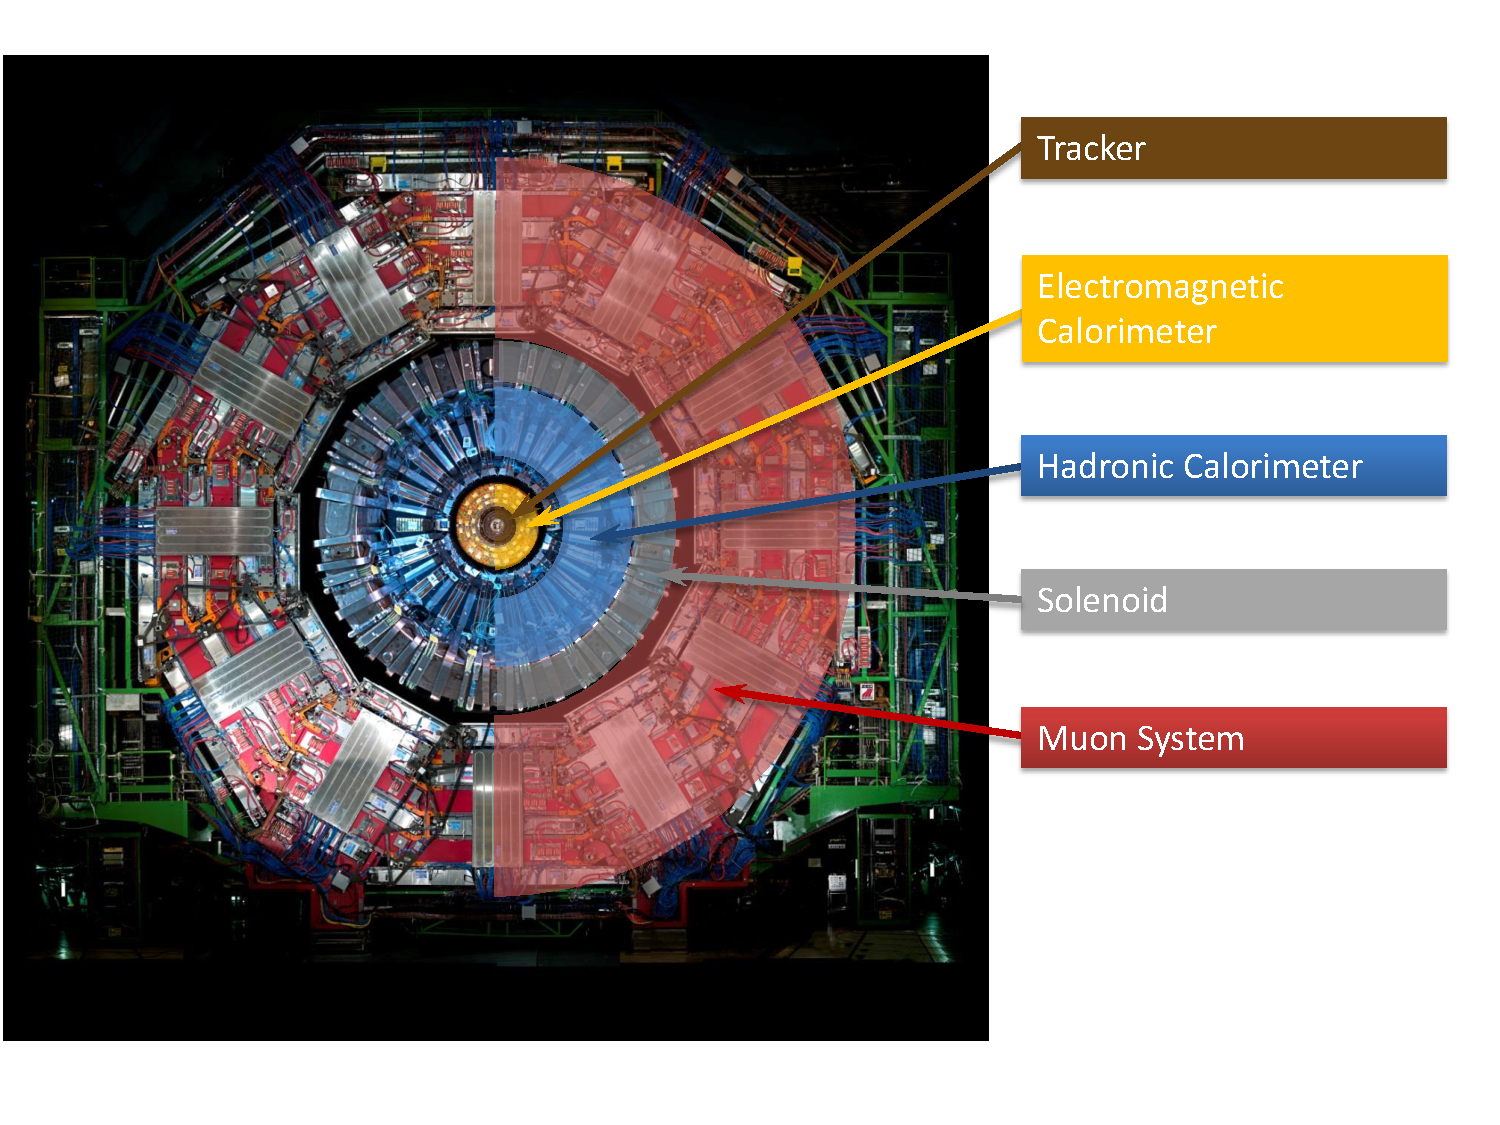
\includegraphics[width=0.99\textwidth]{figures/general/CMS}
 % 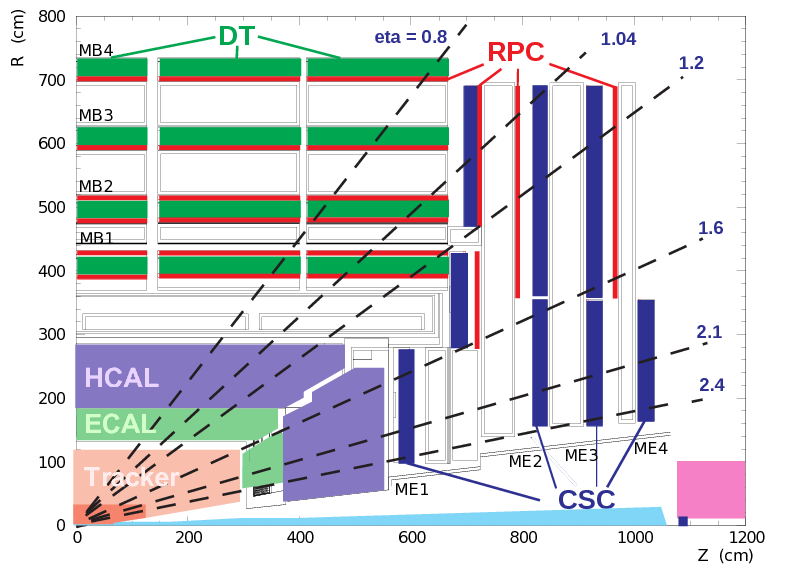
\includegraphics[width=0.49\textwidth]{figures/general/CMS_eta.png}
 \caption{A cross section picture of the open CMS detector~\cite{CMSPicture}. The important parts are labeled.}
 \label{fig:CMS}
\end{figure}

\subsection{Tracker system}
The most inner part of the CMS detector is the inner tracker and it consists of two main components, a silicon pixel and a silicon strip detector\footnote{The silicon pixel detector was replaced at the end of the 2016 run. Since in this thesis only 2016 data is used, only the former detector is described.}. Both components enclose parts parallel to the beam pipe in the barrel, and parts orthogonal to the beam axis in the edncaps. A sketch of the total inner track is shown in \refFig{fig:tracker}. The tracker is designed to allow a precise measurement of particle trajectories and identifiaction of primary and secondary vertices. Therefore, a high granularity and fast response is needed. The silicon pixel subcomponent is built of three barrel layers and two endcap disks, covering a total area size of around $1\m^2$. Each of the $\approx66$ million silicon pixel cells has a size of $100x150\micron^2$. This enables good resolution in all orientations independent of the track direction.\\
The silicon strip detector consists of four strip layers in the inner (TIB), and six layers in the outer part (TOB). In the direction of the endcaps, it is built of three inner disk layers (TID), and nine layer in the outer part (TEC).\\
The inner trackker in total covers a range of $|\eta|<2.5$ and has a size of around $200\m^2$. The performance of the tracker yields a momentum resolution for muons of a transverse momentum of $\approx100\GeV$ of $1-2\%$ in $|\eta|<1.6$. At higher pseudorapidities the momentum resolution decreases due to a lower granularity.

\begin{figure}[hbtp]
 \centering
 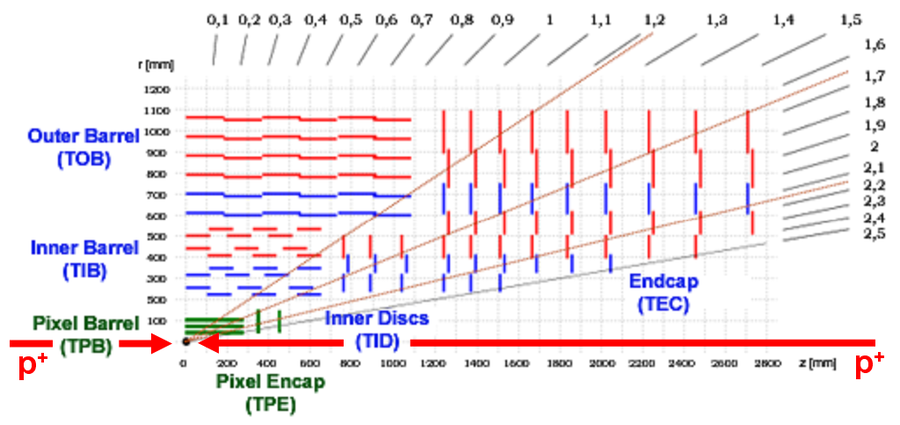
\includegraphics[width=0.69\textwidth]{figures/general/tracker.png}
 \caption{A sketch of one qudrant of the CMS inner tracker~\cite{TrackerPicture}.}
 \label{fig:tracker}
\end{figure}

\subsection{Electromagnetic calorimeter}
\subsection{Hadronic calorimeter}
\subsection{The solenoid}
\subsection{Muon system}
\subsection{Trigger system}
